\documentclass[tikz, border=3mm, ]{standalone}
\usetikzlibrary{arrows.meta,
                decorations.pathreplacing,
                calligraphy,%had to be after lib. decorations.pathreplacing
                positioning,
                shadows
                }
\usepackage{enumitem}
\setlist{nosep,leftmargin=*}

\begin{document}
    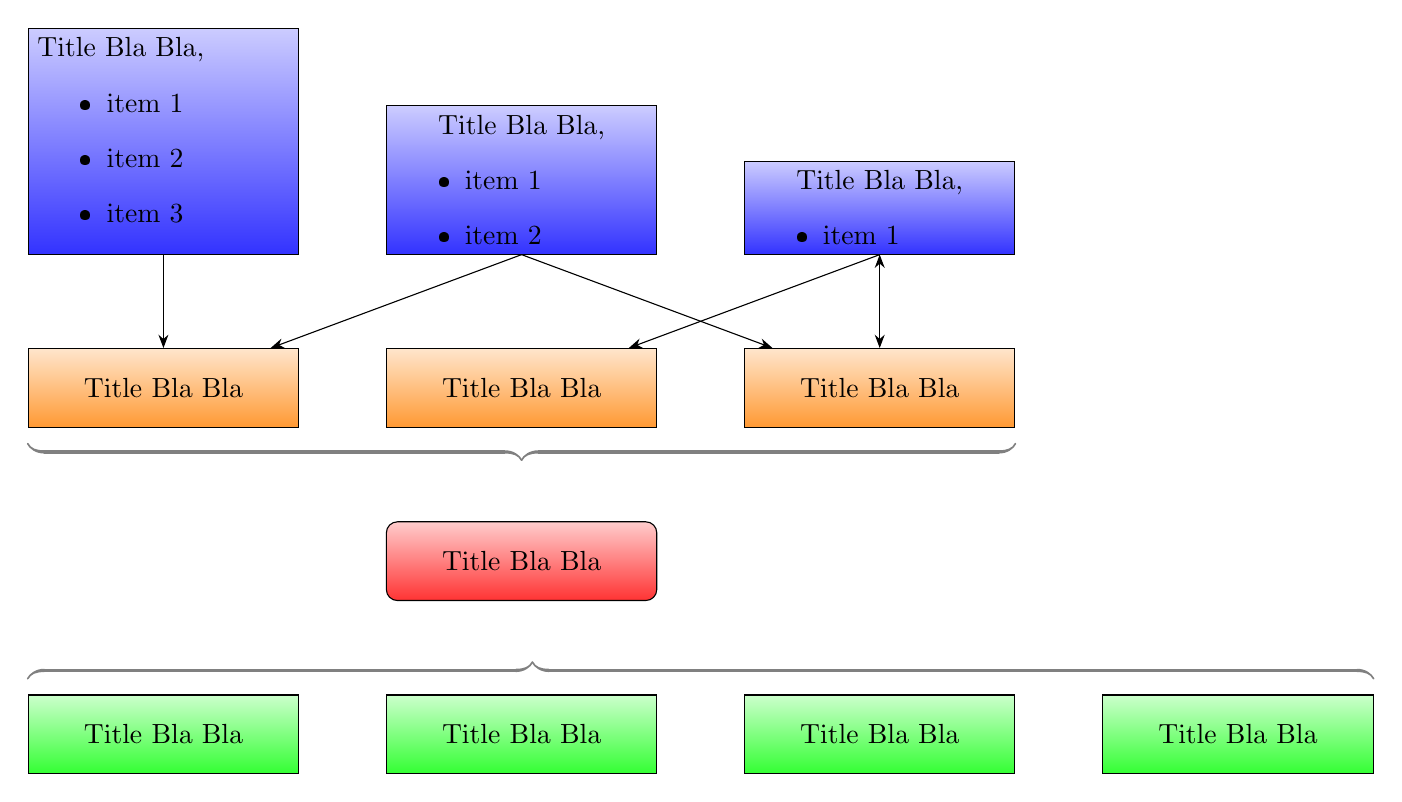
\begin{tikzpicture}[
node distance = 22mm and 11mm,
   box/.style = {shape=rectangle, draw, thin, 
                 minimum height=10mm, text width=32mm, align=center,
                 top color=#1!20, bottom color=#1!80,
                 anchor=south west
                 },
BC/.style args = {#1/#2/#3}{% Braces Calligraphic
        decorate,
        decoration={calligraphic brace, amplitude=6pt,
        raise=#1,
              #2,% for mirroring of brace
        aspect=#3},
        very thick,
        pen colour={gray}
        },
                        ] % mock flow chart
 nodes, first row
\node (start) [box=blue] {\parbox{\hsize}{Title Bla Bla,
                            \begin{itemize}
                        \item   item 1
                        \item   item 2
                        \item   item 3
                            \end{itemize}}};
\node (pro1)  [right=of start.south east,box=blue] {Title Bla Bla,
                            \begin{itemize}
                        \item   item 1
                        \item   item 2
                            \end{itemize}};
\node (pro2)  [right=of pro1.south east,box=blue] {Title Bla Bla,
                            \begin{itemize}
                        \item   item 1
                            \end{itemize}};
% nodes, second row
\node (pro3)  [below=of start.south west,box=orange]    {Title Bla Bla};
\node (pro4)  [right=of pro3.south east,box=orange]     {Title Bla Bla};
\node (pro5)  [right=of pro4.south east,box=orange]     {Title Bla Bla};
% nodes, third row
\node (pro6)  [below=of pro4.south west,box=red,rounded corners] {Title Bla Bla};
% nodes, forth row
\node (pro7)  [below=of pro3.west |- pro6.south,
               box=green]                               {Title Bla Bla};
\node (pro8)  [right=of pro7.south east,box=green]      {Title Bla Bla};
\node (pro9)  [right=of pro8.south east,box=green]      {Title Bla Bla};
\node (pro10) [right=of pro9.south east,box=green]      {Title Bla Bla};
% connections
\draw[-Stealth] (start) edge (pro3)
                (pro1.south)  edge (pro3) (pro1.south)  edge (pro5)
                (pro2.south)  edge (pro4) (pro2.south)  edge (pro5);                
% braces
\draw[BC=2mm/mirror/0.500] (pro3.south west) -- (pro5.south east);
\draw[BC=2mm/      /0.375] (pro7.north west) -- (pro10.north east);
\end{tikzpicture}
\end{document}
